
\chapter{Simulação em hardware}

Com o objectivo de simular a API desenvolvida pretendeu-se encontrar hardware que encaixasse no contexto do problema. Para tal, foram utilizados dois micro-controladores e alguns sensores. Neste capitulo será descrito cada um deles e o processo de desenvolvimento da respetiva simulação.  


\section{Micro-controladores}


Para do cenário anteriormente descrito foram utilizados dois micro-controladores bastante comuns no mercado. Um arduino e um raspberry pi.

\subsection{Arduino Nano}


O Arduino é fruta da evolução de um projeto italiano desenvolvido no ano de 2005, cujo o objetivo consistiu em ser utilizado em projetos escolares de forma a ter um orçamento menor que outros sistemas de prototipagem disponíveis naquela época.

Tal como descrito no seu site oficial, um Arduino consiste numa plataforma \textit{open-source} de prototipagem eletrónica com hardware e software flexíveis e fáceis de serem utilizados. 



Principais características do Arduino Nano: 

\begin{itemize}
	\item Microcontrolador: É o cérebro do Arduino. Este é o dispositivo programável que roda o código que enviamos à placa. Nesta placa o microcontrolador ATmega328 é utilizado, este dispõem de 32kb de memória flash e 2kb de memória ram.
	
	\item  Conector USB: Conector que conecta o Arduino ao computador além de alimentar a placa.
	
	\item  Pinos de Entrada e Saída: Pinos que podem ser programados para agirem como entradas ou saídas fazendo com que o Arduino interaja com o meio externo.
	
	\item Pinos de Alimentação: Fornecem diversos valores de tensão que podem ser utilizados para transmitir energia elétrica aos componentes do seu projeto.
	\item  Botão de Reset: Botão que reinicia o dispositivo.
	\item  Conversor Serial-USB e LEDs TX/RX: O conversor Serial-USB permite que o microcontrolador e o computador se comuniquem, nesta placa o microcontrolador Atmega16U2 é programado para agir como conversor. Os LEDs TX e Rx acendem quando o Arduino está transmitindo e recebendo dados pela porta serial respectivamente.
	\item  Conector de Alimentação: Permite com que uma fonte alimente a placa. Caso o Arduino esteja sendo alimentado pela porta USB e por uma fonte o hardware seletor escolherá automaticamente a melhor fonte.
	\item LED de Alimentação: Indica se a placa está a transmitir energia.
	\item LED Interno: LED ligado ao pino digital 13.
	
	
	
\end{itemize}




\begin{table}[h]
	\centering
	
	\begin{tabular}{|
			>{\columncolor[HTML]{C0C0C0}}l |l|} \hline
		Microcontrolador & ATmega328 \\ \hline
		Tensão de Operação & 5V \\ \hline
		Tensão de Entrada & 7-12V \\ \hline
		Portas Digitais & 14 (6 podem ser usadas como PWM) \\ \hline
		Portas Analógicas & 8 \\ \hline
		Corrente Pinos I/O & 40mA \\ \hline
		Memória Flash & 32KB (2KB usado no bootloader) \\ \hline
		SRAM & 2KB \\ \hline
		EEPROM & 1KB \\ \hline
		Velocidade do Clock & 16MHz \\ \hline
		Dimensões & 45 x 18mm \\ \hline
	\end{tabular}
	\caption{Características do sensor TTC 104}
	\label{my-label}
\end{table}


O que pode ser feito? 
Evolução... 

Componentes
IDE



\begin{figure}[h]
	\centering
	\begin{minipage}[b]{0.4\textwidth}
		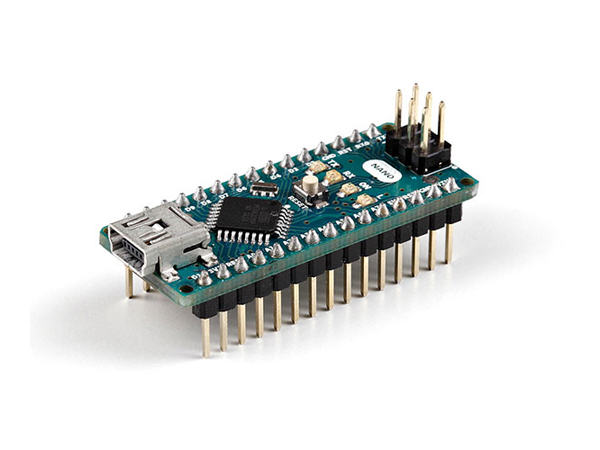
\includegraphics[width=\textwidth]{img/hardware/nano-img.jpg}
		\caption{Flower one.}
	\end{minipage}
	\hfill
	\begin{minipage}[b]{0.3\textwidth}
		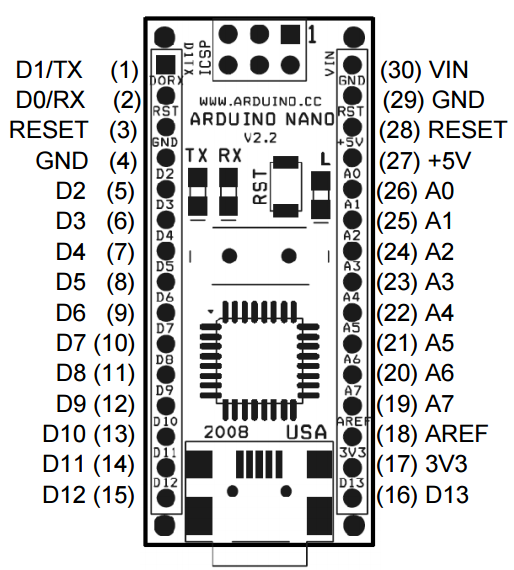
\includegraphics[width=\textwidth]{img/hardware/nano-esquema.png}
		\caption{Flower two.}
	\end{minipage}
\end{figure}


https://www.arduino.cc/en/uploads/Main/ArduinoNanoManual23.pdf


\newpage

\subsection{Raspberry pi }


\begin{figure}[h]
	\centering
	\begin{minipage}[b]{0.4\textwidth}
		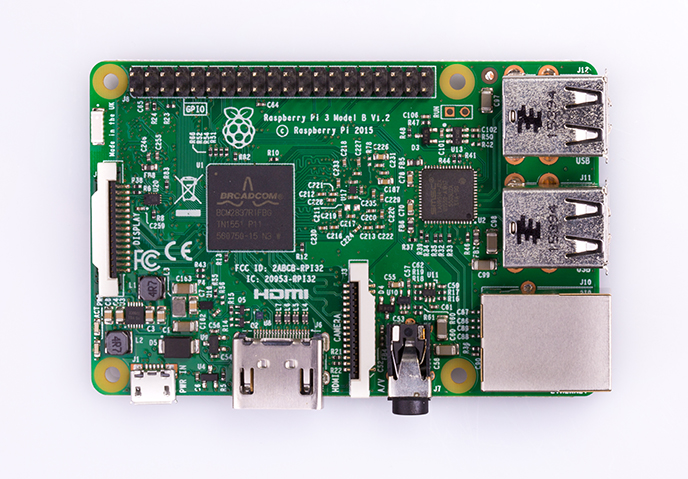
\includegraphics[width=\textwidth]{img/hardware/rasp3-img.jpg}
		\caption{Flower one.}
	\end{minipage}
	\hfill
	\begin{minipage}[b]{0.4\textwidth}
		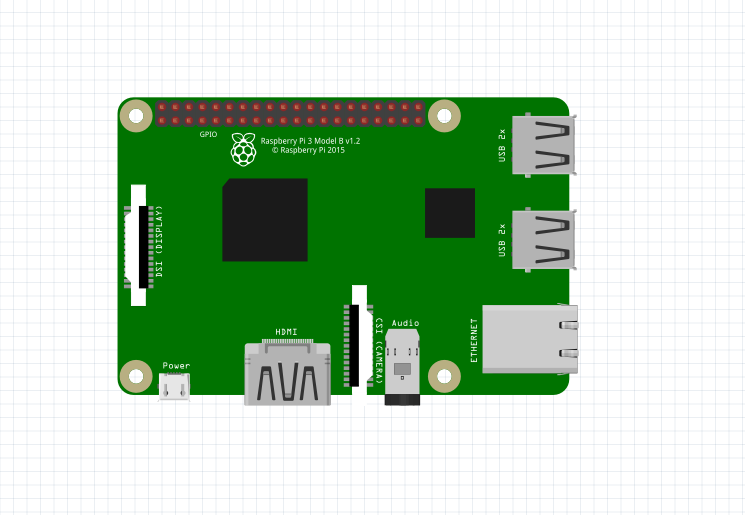
\includegraphics[width=\textwidth]{img/hardware/rasp-esquema.PNG}
		\caption{Flower two.}
	\end{minipage}
\end{figure}


\newpage
\section{Interligação de componentes}




\section{Considerações finais}
